\section{Concepts}
\label{sec:concepts}

The Generator framework provides:

* A toolbar button to initiate the generation
* Generic code to remove previously generated elements
* Generic code to organise the incorporation of newly generated elements
* Utilities to aid the creation of new elements
* An abstract basis for client defined rules
* An extension point for clients to declare generators and generation rules

The client rules return generation descriptors (rather than modifying the target model directly). The framework takes care of updating the model (within the clients Transactional Editing Domain) provided the generation completes successfully. This ensures that the model is not left in an inconsistent state should the generation fail. The generation descriptors allow the client to specify where the new element should be contained and a priority which will be used to influence the placement of the new element within the containment ordering.

To define a particular generator a client should:

* Define an extension of org.eclipse.ui.handlers to enable the generate command when the activePartID is their Editor (see [[Defining a generator handler]])
* Define an extension of ac.soton.eventb.emf.diagrams.generator.rule to make the generator framework aware of your generator and its rule classes.
* Implement your rule classes

\subsection{Adapter}
\label{sec:adapter}

\texttt{<TO BE WRITTEN>}

\subsection{Generation Descriptors}
\label{sec:descriptors}

Each rule should return a collection of one or more Generation Descriptors. Generation Descriptors have the following fields which are explained in this section.

* EventBElement parent;
* EStructuralFeature feature;
* Object value;
* Integer priority;
* Boolean editable;
* Boolean remove;

The feature of the parent will be changed in the following ways:

If remove is false:
* 1) If the feature is a containment and the value is an element of the correct kind, the value will be added to the containment in a position according to the priority
* 2) If the feature is a reference and the value is an element of the correct kind, the value will be added to the reference in a position according to the priority
* 3) If the feature is an EAttribute and the value is of the correct type, the feature will be set to the value

Priority can be used to control the relative position of the generated elements  
* 1 - must come first
* 10 - not important
* ---user entered items---
* 0 must come after user entered items
* -10 must come last

Editable - this affects read-only status of the generated element and whether or not it will be preserved or re-generated in a subsequent generation.
* false - the element is set as read-only (the user cannot change its attributes nor add/remove children), any existing copy of the element will be deleted and re-generated at each re-generation
* true  - the element is not read-only and will not be deleted before re-generation. (N.B. It is the responsibility of the client rules to check whether this element already exists and only only generate a new one if it does not)

If remove is true:
* 1) If the feature is a containment and the value is an element of the correct kind, the value will be deleted from the containment
* 2) If the feature is a reference and the value is an element of the correct kind, the value will be removed from the reference
* 3) If the feature is an EAttribute, the feature will be unset 

\subsection{Rules}
\label{sec:rules}

Rule classes must implement IRule. It is recommended the rule classes extend
 \begin{verbatim}
 ac.soton.eventb.emf.diagrams.generator#AbstractRule
 \end{verbatim}
 which provides some concise constants for the commonly needed containments and defines some default behaviour (always enabled and dependencies ok).  Note that the rule will only be attempted for the type of source element defined in the extension point. However, this could be defined as an abstract base class to allow the rule to operate on several types of element.

Where a tree structure is entirely generated within one rule firing (e.g. an event with guards and actions) it is more efficient to construct the entire event and return a single Generation Descriptor that adds that event. It is also possible to do this by returning separate Generation Descriptors to add the event and each guard and action individually. Using a single descriptor is more efficient but means that some features of the translator framework are bypassed. For example, the priority scheme cannot be used, your code will determine the order. 

A typical line from a rule class might look like this:
 \begin{verbatim}
 ret.add(Make.descriptor(machine,invariants,
			Make.invariant("myInvariantName", "myVar >0","my comment")
			,10));
 \end{verbatim}		
where,  ret is the list to be returned and machine is the parent element containing the invariants to be added to.

A rule has 4 methods:
\begin{itemize}
\item \texttt{boolean enabled (final EventBElement sourceElement)}
\item \texttt{boolean dependenciesOK(EventBElement sourceElement, \\  List<GenerationDescriptor> generatedElements)}
\item \texttt{boolean fireLate()}
\item \texttt{List<GenerationDescriptor> fire(EventBElement sourceElement, \\   List<GenerationDescriptor> generatedElements)}
\end{itemize}

The \textbf{enabled} method can be used to restrict when it applies. More than one rule can be defined for the same kind of element allowing the generation to be decomposed in a maintainable way. 

The \textbf{DependenciesOK} method allows the method to be deferred since the success of rules may depend on what has already been generated. The dependenciesOK method is passed the list of GenerationDescriptors created so far.

The \textbf{fireLate} method forces the rule to be fired when all other rules have been fired. This is usually used when the rules behaviour depends on what other rules have done.

The \textbf{fire} method must return a list of GenerationDescriptors describing what should be generated. The Utility class, Make, provides a convenience method to help construct a GenerationDescriptor from the parent element, the containment feature, the new child and the priority indicator and if needed the editable setting.

\subsection{Priorities}
\label{sec:priorities}

Priority may be from 10 to -10, where 1 indicates first in the containment and -10 last in the containment. Elements in the containment that are not (currently) being generated are placed between priorities 10 and 0. Bear in mind that the relative position of different diagrams (extensions) is preserved within each priority band. Also the order of source elements within their containment is preserved within each priority band.

\begin{verbatim}
1 2 3 4 5 6 7 8 9 10 <other content> 0 -1 -2 -3 -4 -5 -6 -7 -8 -9 -10
\end{verbatim}

For example, a basic type invariant that doesnt depend on other variables might be placed at position 1 whereas a theorem or invariant included purely for proof purposes might be placed at position -10. 

A current limitation of the priority scheme is that there are a limited number of priorities. For example, this could be a problem if a rule needs to calculate positions of each element within a collection based on dependencies of the element instance.

\subsection{Editable}
\label{sec:editable}
In most cases the generated element should be set as non-editable (the default). In this case the element will be deleted and re-generated on each invocation of the generator. The user should not change any attributes of the element nor add to its children. In some case, however, it is necessary to generate an element whose contents may be modified by the user. To do this set the editable parameter of the Generation Descriptor. In this case the generated element will not be deleted when the generator is next invoked. The rule must take care not to return another Generation Descriptor if the element has already been generated. It should look for a suitable generated element (to use for adding further generated chldren etc.) and only generate a new one if it doesn't exist.

%
%\subsection{Example Figure}
%\label{sec:xtext-projects}
%
% A figure (see Figure~\ref{fig:XContextPreference}.
%\begin{figure}[!htbp]
%  \centering
%  \ifplastex
%  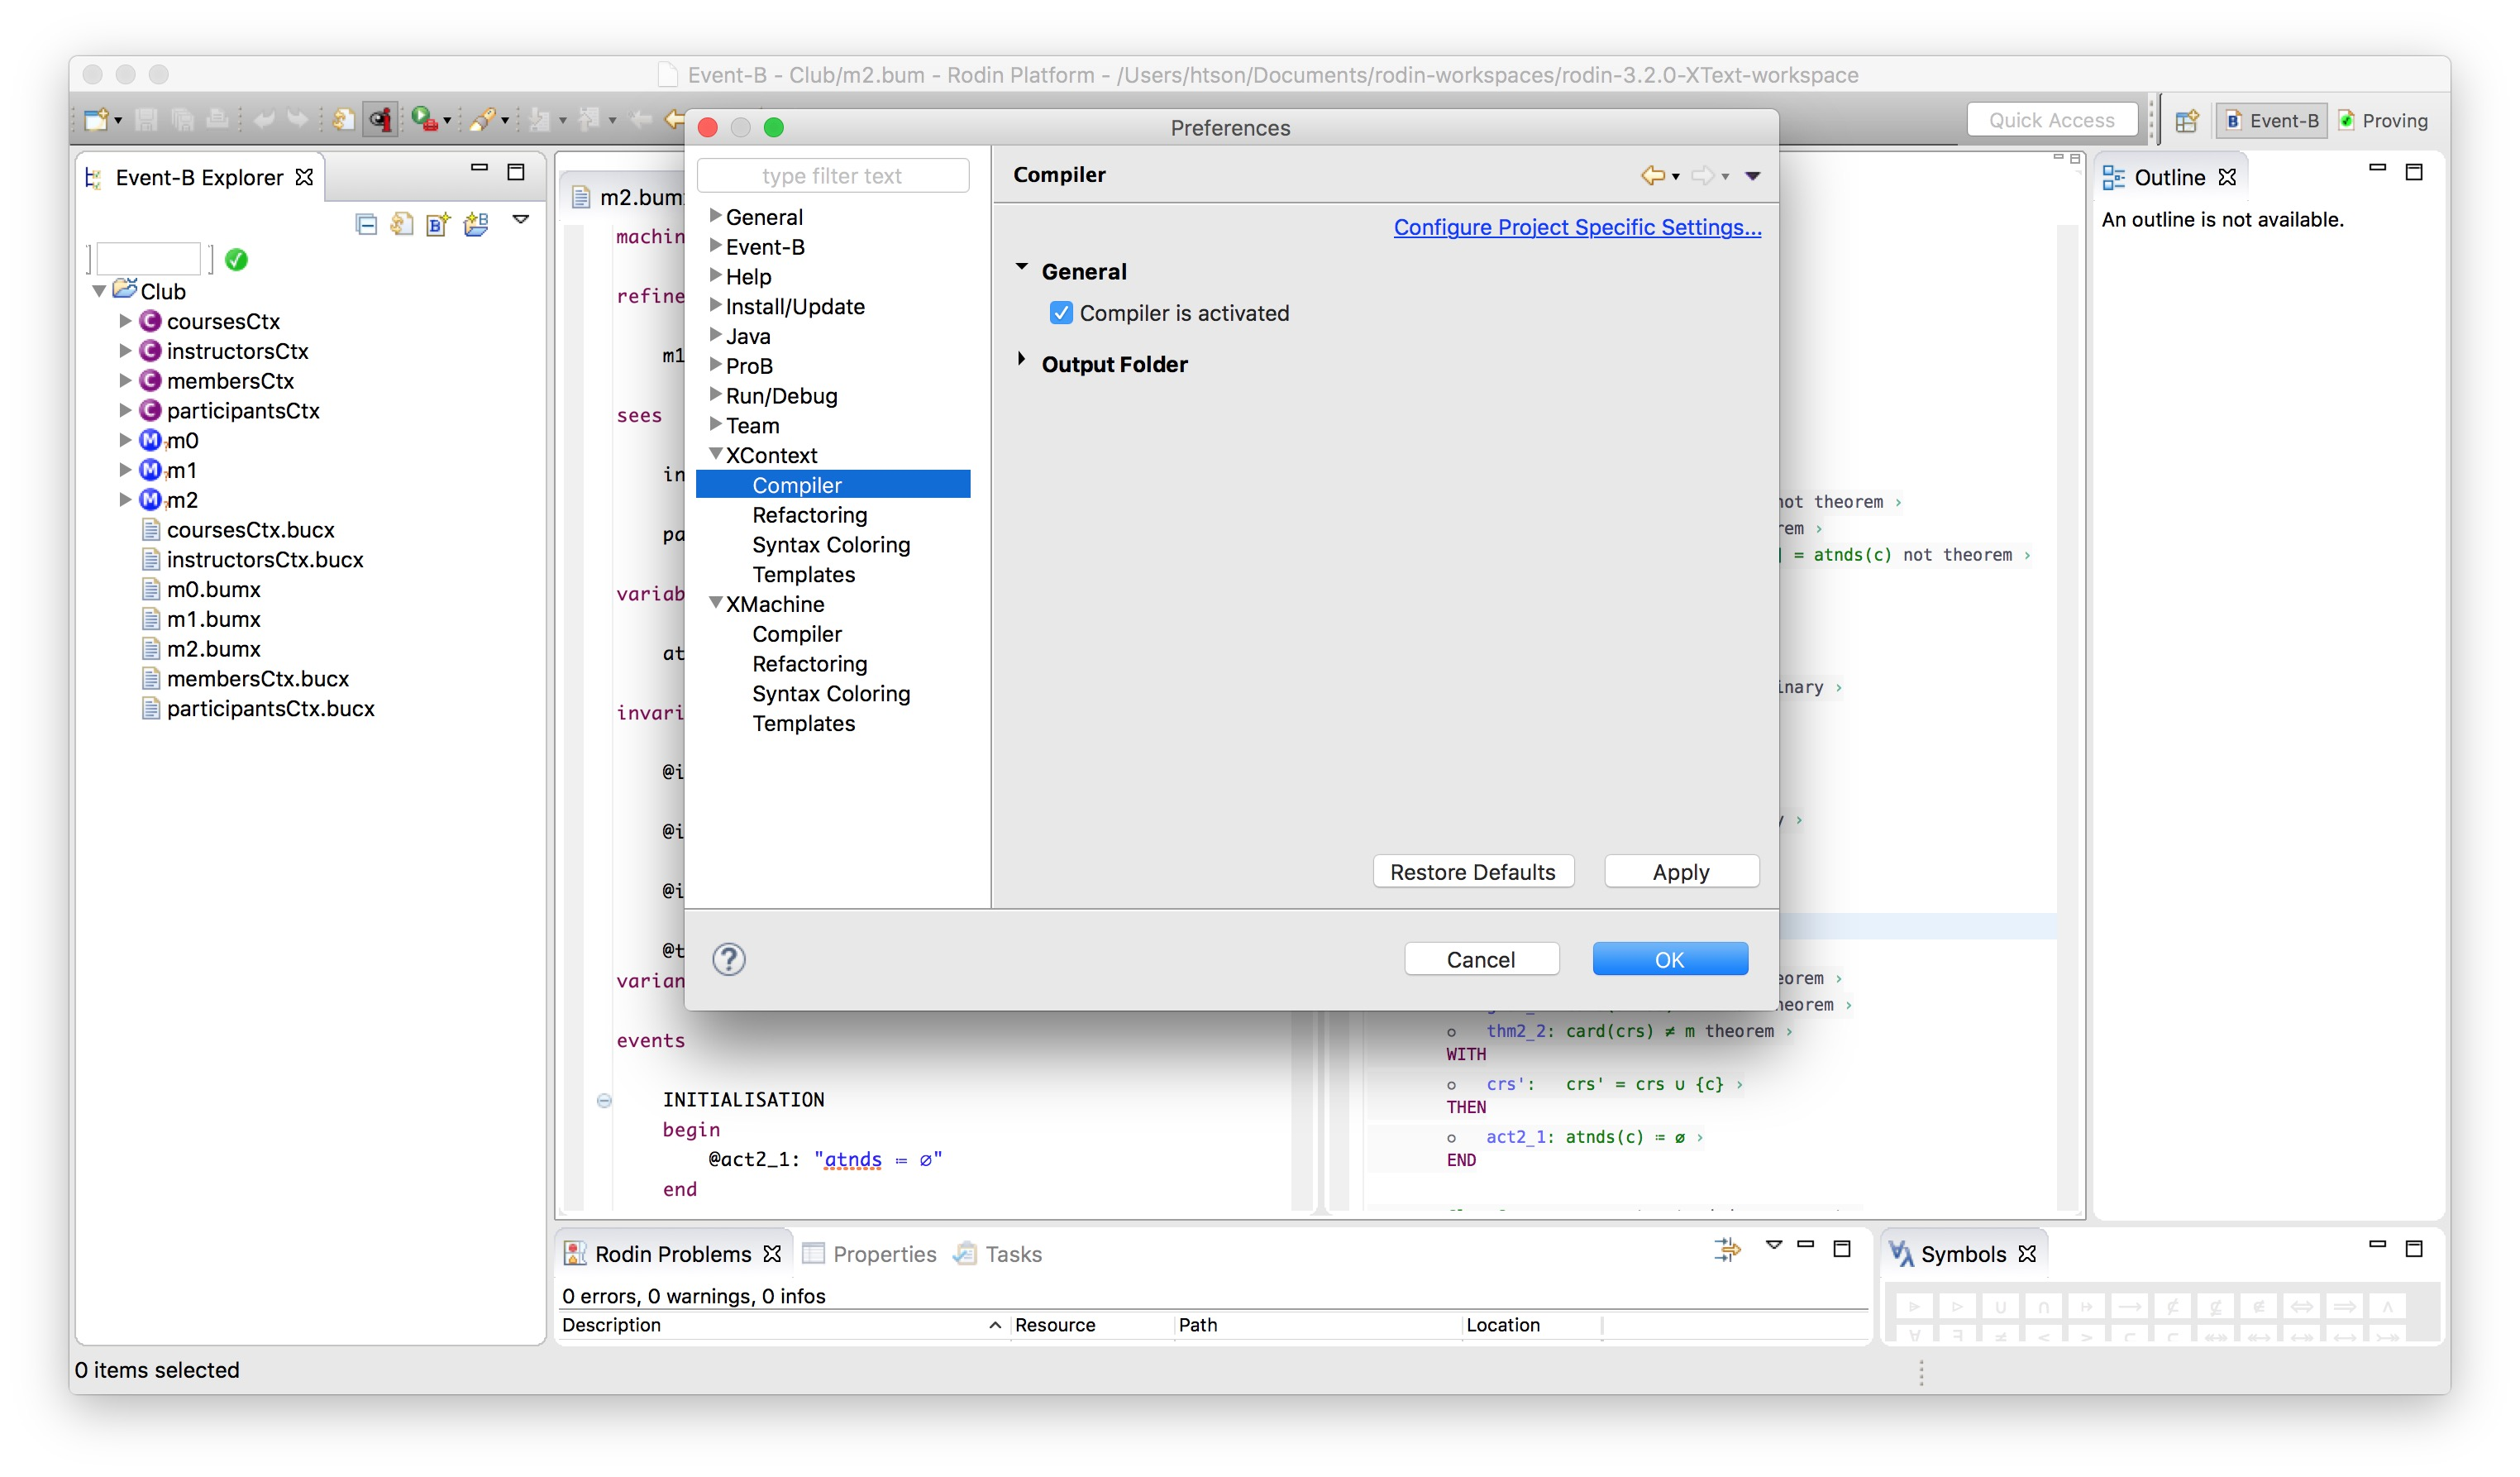
\includegraphics[width=512]{figures/XContextPreference}
%  \else
%  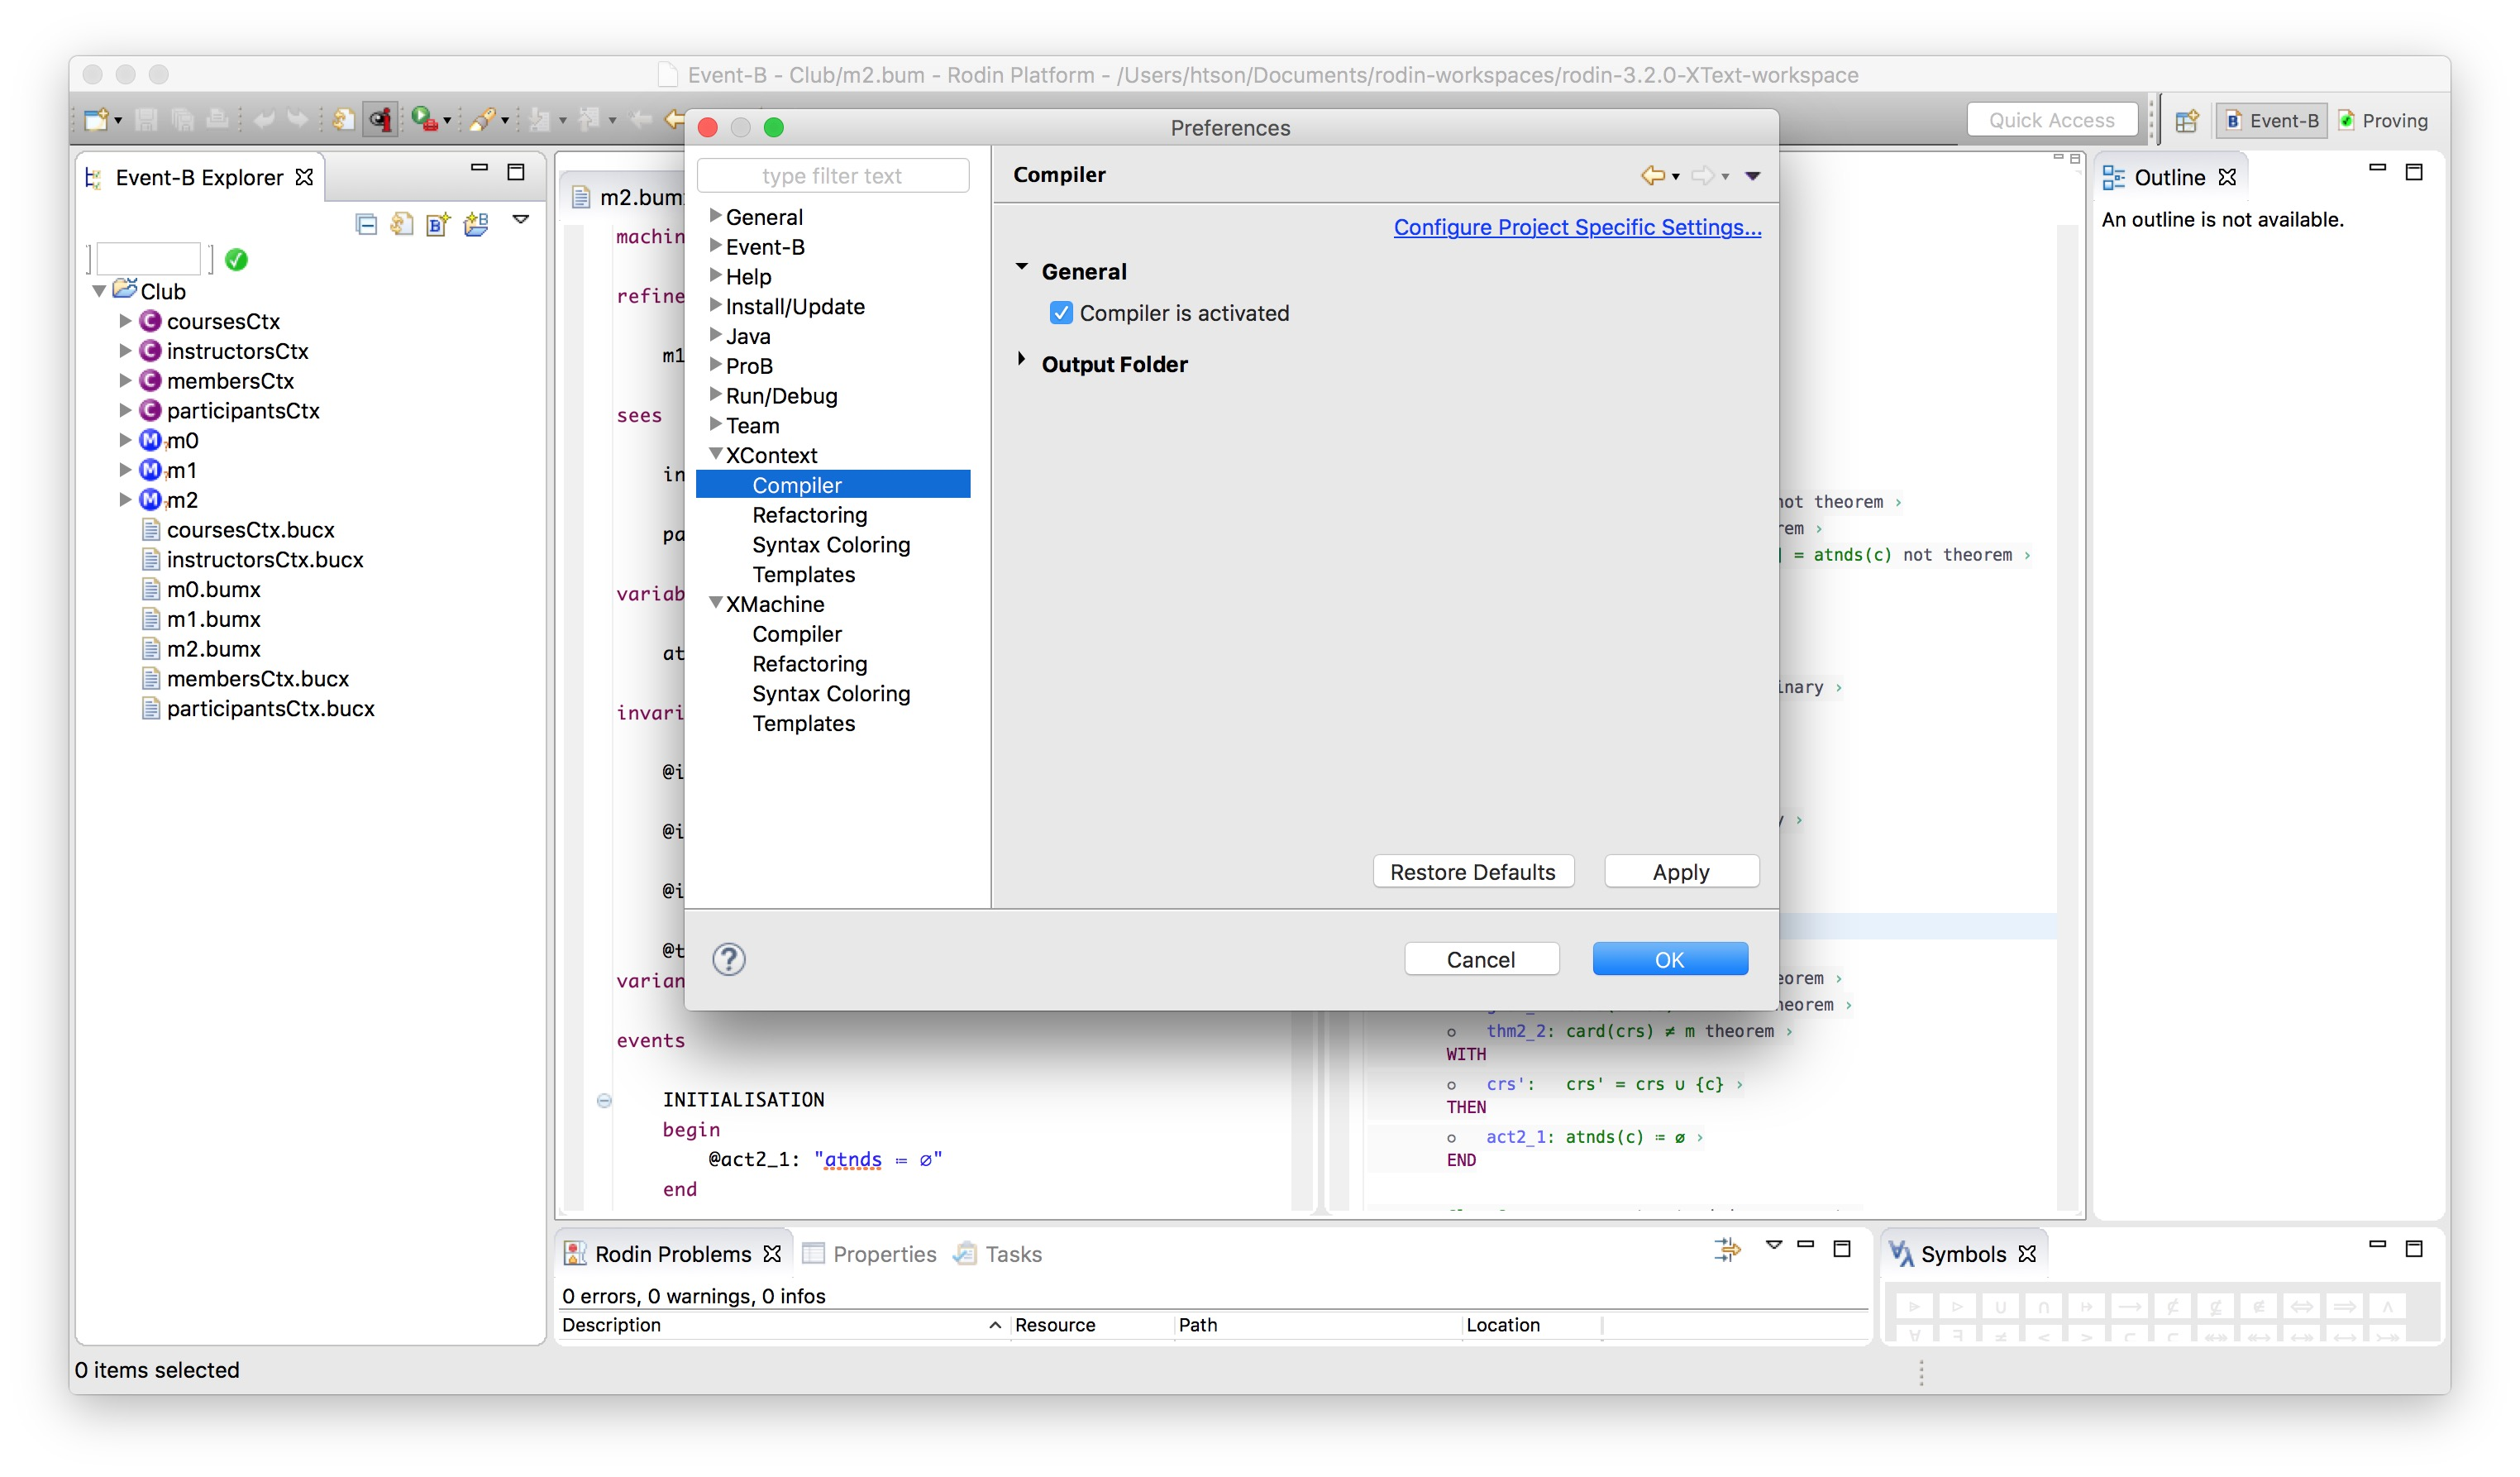
\includegraphics[width=0.9\textwidth]{figures/XContextPreference}
%  \fi
%  \caption{XContext Preference}
%  \label{fig:XContextPreference}
%\end{figure}


%%% Local Variables:
%%% mode: latex
%%% TeX-master: "user_manual"
%%% End:
